\section {Was is WebBrick?}

A WebBrick is a process control device with a network interface.  The process control is implemented by state engines that accept
triggers \index{trigger} from a variety of sources and control an output according to the state engine's configuration.

For example, an engine may accept a trigger from trigger input 0 and then hold digital output 7 high for 30 seconds.

This engine could also be triggered from at HTTP request via the embedded web site, or from a UDP packet.

The WebBrick has 8 trigger inputs, 1 analogue input, 1 temperature input, 1 rotary encoder input, 8 digital output and two analogue outputs.

\begin{figure}[H]
\centering
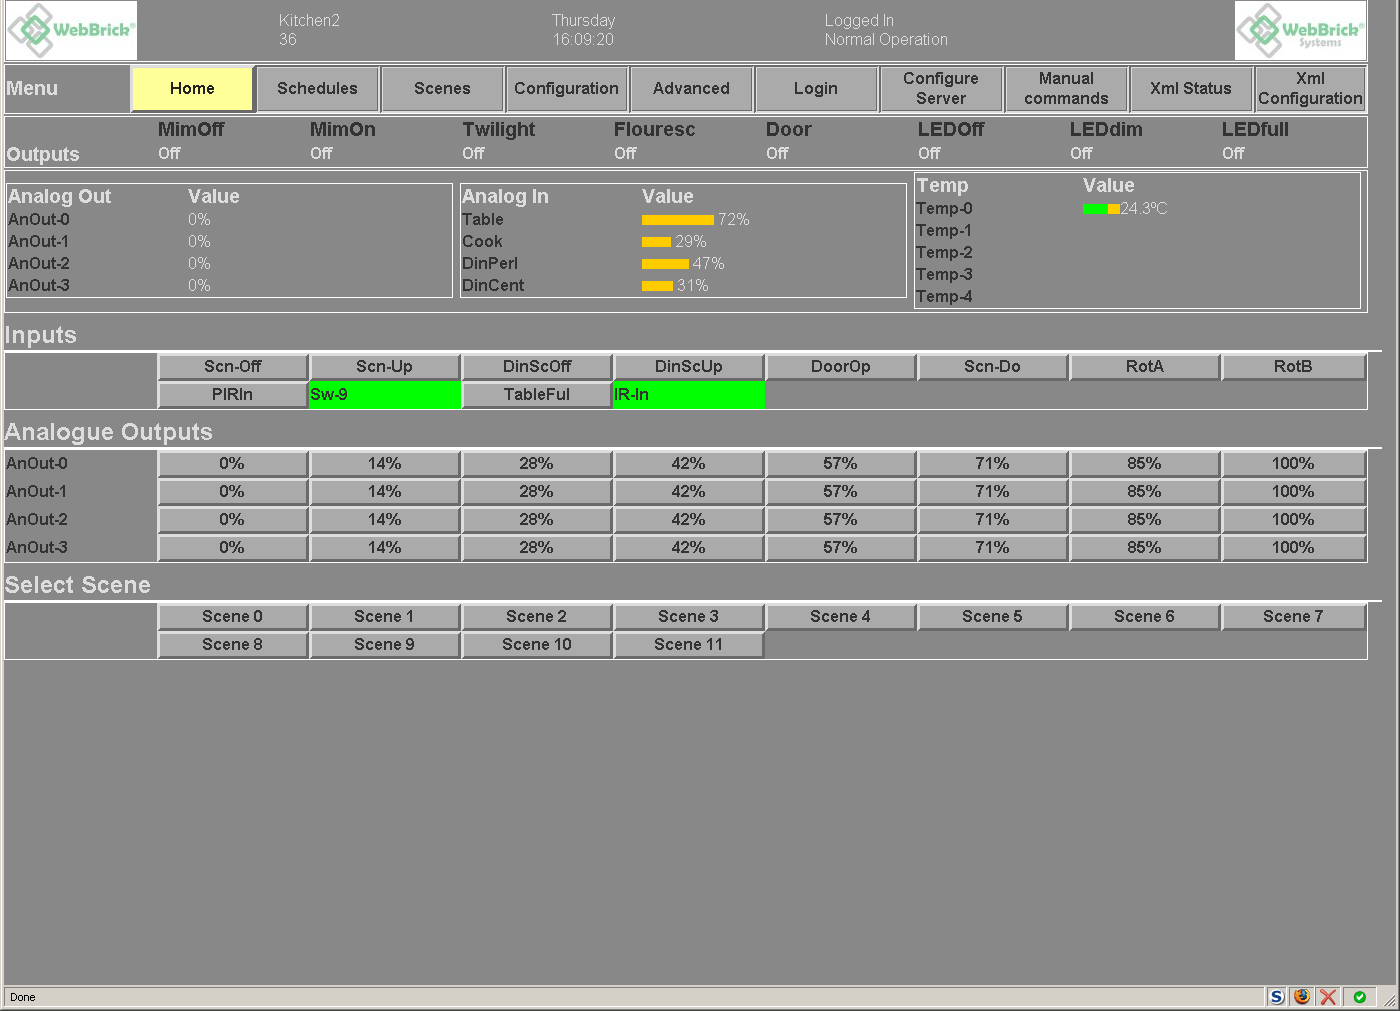
\includegraphics[width=1.0\textwidth]{Images/home.jpg}
\end{figure}

\subsection{State engines}

\index{State engines}

    The state engines are what give the WebBrick its ability to do local control whilst allowing the interaction of global intelligence.  In essence one a Trigger is invoked it will carry out the actions specified until the actions are complete, or there is an intervention from another Trigger or remote command.
    
    \begin{figure}[H]
    \centering
    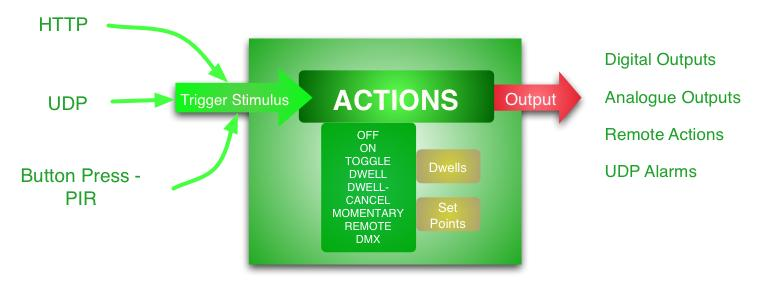
\includegraphics[width=0.9\textwidth]{Images/StateEngineDiag.jpg}
    \end{figure}
    
    More than one Trigger can action an output.  For example there might be conditions that say switch a light on, and some that turn it off.
    
\subsection{Using WebBrick}

    WebBricks can be valuable even in a non-networked environment.  This section shows how the WebBrick can be used:
    \begin{itemize}
    \item as a standalone device
    \item as part of a network with other WebBricks
    \item as part of a network with generic hosts providing some 'global intelligence'
    \end{itemize}
    
    In the following sections, some of the concepts of the WebBrick are introduced.  The full format of specific commands are documented
    later in this manual.

\subsubsection{As a standalone device}

\index{WebBrick as Standalone device}

Consider that you have an ensuite bathroom with dimmable halogen downlights, lights around a mirror, and a heated floor.

In this case the WebBrick would be temporarily connected to a PC to configure the state engines, the configuration might look like this:

\begin{description}
\item[Trigger 0]  This would be set to perform a \textbf {Dwell-Cancel} of 1 hour on the digital output connected to the heated floor.
\item[Trigger 1]  This would be set to perform a \textbf {Toggle} of the digital output connected to the mirror lights
\item[Trigger 2]  This would be set to perform a \textbf {Toggle to-from 25\% } of analogue output 0, which would control the halogen downlights
\item[RotStep]  This would be set to 8 so that a standard 16 indent rotary encoder could set analogue output 0 to 0-100\% in one rotation
\item[Temperature]  This would be set to perform a \textbf {Off} above 35degC ofthe digital output connected to the heated floor
\end{description}

Now the WebBrick can be taken to the location and connected:

\begin{description}
\item[Trigger 0 - Heated Floor]  To a push button with LED within the ensuite
\item[Trigger 1 - Mirror Lights] To a push button with LED within the ensuite
\item[Trigger 2 - Main Lights]  To a push button with LED within the bedroom (within reach of the bed)
\item[Digital Output 0 high] To a solid state relay (SSR) that powers the heated floor
\item[Digital Output 0 low] To the LED for the push button of Trigger 0
\item[Digital Output 1 high] To a SSR that powers the mirror lights
\item[Digital Output 1 low] To the LED for the push button of Trigger 1
\item[Rotary Encode]  To a rotary encoder within the ensuite
\item[Temperature]  To a Dallas 1821 'One Wire' temperature sensor that is bonded to the heated floor at a convienent point
\item[Analogue Output 0] To a 0-10V dimmer that controls the Halogen downlight. Also to the LED of push button within the bedroom
\end{description}

So what does this give the human users?  First they have convienent, safe low voltage controls for switching the lights and the heated floor.
Second from within the bedroom they have a way of switching the ensuite lighting either off from any level or, switching it on to a low level
enough to see by, but not to blind.  By adding a second push button in parallel with Trigger 0 they can both see and switch the state of the
heated floor within the ensuite.

Note that the \textbf{Dwell-Cancel} is used so that should the floor button be pressed, the floor will stay on for 1 hour, unless the button is pressed
again within the hour, in which case the 'dwell' will be cancelled and the heated floor switched off.  This is useful for people that might forget
to switch the floor off, and those that would like to switch the floor off as soon as they are done to save energy.

The configuration of the temperature sensor is used to provide a safety cut-out should the temperature of the heated floor get too high.

\subsubsection{More than one WebBrick on a network}

\index{Multiple WebBricks on a network}

Consider our bedroom and ensuite example from above and add the idea that we have another WebBrick in the kitchen and that the two are networked together.
imagine that the kitchen has a heated floor and that the people might like to control the floor from the bedroom.  They might like to do this so that the
floor is warm before they get to the kitchen.

The kitchen WebBrick would have a similar configuration, with a push button creating a \textbf{Dwell-Cancel} for 1 hour.  It would also use a second trigger
as a \textbf{Dwell} for the same digital output channel.  This second trigger would not be connected to any push button.

Using a push button connected to the ensuite WebBrick say Trigger 3, Trigger 3 would be configured to send a \textbf{remote UDP} command to the \textbf{Dwell}
trigger of the kitchen WebBrick.  Pressing this button would ensure that no matter what the current state of the kitchen heated floor, it would start a dwell of 1 hour.

The dwell created by the remote command can be cancelled with the local push button in the kitchen.

\subsubsection{Using the WebBricks with 'global intelligence'}

Lets take our ensuite/bedroom/kitchen example a little further.  Consider that a computer was available that could support a web server
and the PHP and Python langauges. In practice this means most commonly used systems, from linux on an X-Box to Windows 2003 Server on a PC.

Some sample XML configured web-sites and a series of {\em Public Domain} functions and examples are available in both PHP and Python.  These allow for configuration, operation and monitoring of WebBricks.

The host could use a combination of these functions to find out what was going on at the WebBrick and to send commands to them.

For example, regularly scheduled jobs could be used to switch the heated floor on before the occupants wake up.  Note that for the occupants
this is a convience, and all the physical push button controls still work and can always be used to override the remote commands.

Using simple web browsers, extra interfaces can be created that allow users to control their floors and lights.  By using SMS services from TextAnywhere we can extend the controls to the mobile phones that our users carry about.



